\documentclass[11pt,letterpaper]{article}

\newenvironment{proof}{\noindent{\bf Proof:}}{\qed\bigskip}

\newtheorem{theorem}{Theorem}
\newtheorem{corollary}{Corollary}
\newtheorem{lemma}{Lemma} 
\newtheorem{claim}{Claim}
\newtheorem{fact}{Fact}
\newtheorem{definition}{Definition}
\newtheorem{assumption}{Assumption}
\newtheorem{observation}{Observation}
\newtheorem{example}{Example}
\newcommand{\qed}{\rule{7pt}{7pt}}

\newcommand{\solution}[4]{
\thispagestyle{plain} 
\newpage
\setcounter{page}{1}
\noindent
\begin{center}
\framebox{ \vbox{
\vspace{4mm}
\vspace{0.2in} 
{\centering \large\mbox{#3}}\\
\vspace{0.1in}
{#1 \hfill {Date: #2}}
}}
\end{center}
\markright{#1}
}

\newenvironment{algorithm}
{\begin{center}
\begin{tabular}{|l|}
\hline
\begin{minipage}{1in}
\begin{tabbing}
\quad\=\qquad\=\qquad\=\qquad\=\qquad\=\qquad\=\qquad\=\kill}
{\end{tabbing}
\end{minipage} \\
\hline
\end{tabular}
\end{center}}

\def\Comment#1{\textsf{\textsl{$\langle\!\langle$#1\/$\rangle\!\rangle$}}}



\usepackage{graphicx, amssymb, amsmath, listings, float, mathtools}
\usepackage{color, url}
\lstset{language = Python}
\lstset{breaklines}
\lstset{extendedchars=false}

\oddsidemargin 0in
\evensidemargin 0in
\textwidth 6.5in
\topmargin -0.6in
\textheight 9.0in

\begin{document}

\solution{\large Jifu Zhao}{\large 09/30/2016}{\bf \Large ECE 544NA \hspace{0.5cm} 
		Fall 2016 \hspace{0.5cm} Assignment 2}

\section*{\Large I. Pencil-and-Paper}
\begin{description}
%%%%%%%%%%%%%%%%%%%%%%%%%%%%%%%%%%%%%%%%%%%%%%%%%%%%%%%%%%%%%%%%%%%%%%%%%%%%%%%%%%%%%%%%%
% Problem 1
\item{\bf \large 1. } Derivative of Softmax \\
Recall the softmax function:
\begin{equation}
	\vec{y}[k] = \frac{e^{\vec{z}[k]}}{\sum_{l=1}^C e^{\vec{z}[l]}}
\end{equation}

So, consider two cases, j = k and j != k. 

When j = k:
\begin{equation}
	\frac{\partial \vec{y}[k]}{\partial \vec{z}[j]} 
		= - \frac{e^{\vec{z}[k]} \cdot \sum_{l=1}^C e^{\vec{z}[l]} - e^{\vec{z}[k]} \cdot e^{\vec{z}[k]}} 
				{(\sum_{l=1}^C e^{\vec{z}[l]})^2}
		= \vec{y}[k] - \vec{y}[k] \cdot \vec{y}[k]
\end{equation}

When j != k:
\begin{equation}
	\frac{\partial \vec{y}[k]}{\partial \vec{z}[j]} 
		= - \frac{e^{\vec{z}[k]} \cdot e^{\vec{z}[j]}} 
				{(\sum_{l=1}^C e^{\vec{z}[l]})^2}
		= - \vec{y}[k] \cdot \vec{y}[j]
\end{equation}

So, we can conclude that:
\begin{equation}
	\frac{\partial \vec{y}[k]}{\partial \vec{z}[j]} = 
	\begin{cases}
		- \vec{y}[k] \cdot \vec{y}[j]				& \quad \text{if } k != j \\
		\vec{y}[k] - \vec{y}[k] \cdot \vec{y}[k]	& \quad \text{if } k = j \\
	\end{cases}
\end{equation}


%%%%%%%%%%%%%%%%%%%%%%%%%%%%%%%%%%%%%%%%%%%%%%%%%%%%%%%%%%%%%%%%%%%%%%%%%%%%%%%%%%%%%%%%%
% Problem 2
\item{\bf \large 2. } Negative Log Likelihood loss for Multi-Class. \\
Recall the negative log likelihood: 
\begin{equation}
	L = - \sum_i^N \sum_k^K {\bf 1}[y_i = k] \cdot log(\hat{\vec{y}}_i[k])
\end{equation}

In this way, we have:
\begin{equation}
	\frac{\partial L}{\partial \hat{\vec{y}}_i[j]} 
	= - {\bf 1}[y_i = k] \cdot \frac{\partial log(\hat{\vec{y}}_i[j])}{\partial \hat{\vec{y}}_i[j]}
	= - \frac{{\bf 1}[y_i = j]}{\hat{\vec{y}}_i[j]}
\end{equation}


%%%%%%%%%%%%%%%%%%%%%%%%%%%%%%%%%%%%%%%%%%%%%%%%%%%%%%%%%%%%%%%%%%%%%%%%%%%%%%%%%%%%%%%%%
% Problem 3
\item{\bf \large 3. } Avg-pooling (1D) \\
Recall Avg-pooling (1D) operation with window size W: 
\begin{equation}
	\vec{y}[i] = \frac{1}{W} \sum_{j=0}^W \vec{x}[i + j]
\end{equation}

Then, we have:
\begin{equation}
	\frac{\partial \vec{y}[i]}{\partial \vec{x}[j]} = 
		\begin{cases}
			- \frac{1}{W}	& \quad \text{if } i \leq j \leq i + W \\
			0				& \quad \text{otherwise} \\
		\end{cases}
\end{equation}

%%%%%%%%%%%%%%%%%%%%%%%%%%%%%%%%%%%%%%%%%%%%%%%%%%%%%%%%%%%%%%%%%%%%%%%%%%%%%%%%%%%%%%%%%
% Problem 4
\item{\bf \large 4. } Max-pooling (1D) \\
Recall Max-pooling (1D) operation with window size W: 
\begin{equation}
	\vec{y}[i] = \max_{j=0}^W \vec{x}[i + j]
\end{equation}

Then, we have:
\begin{equation}
	\frac{\partial \vec{y}[i]}{\partial \vec{x}[j]} = 
		\begin{cases}
			1	& 	\quad \text{if } \max_{k=0}^W \vec{x}[i + k] = \vec{x}[j] \\
			0	& 	\quad \text{otherwise} \\
		\end{cases}
\end{equation}


%%%%%%%%%%%%%%%%%%%%%%%%%%%%%%%%%%%%%%%%%%%%%%%%%%%%%%%%%%%%%%%%%%%%%%%%%%%%%%%%%%%%%%%%%
% Problem 5
\item{\bf \large 5. } Convolutional layer (1D)\\
Recall Convolution (1D) operation, assume $\vec{w}$ is length 3, and zero index at the center:
\begin{equation}
	\vec{y}[i] = (\vec{w} \ast \vec{x})[i] = \sum_{j=-1}^1 \vec{x}[i-j] \cdot \vec{x}[j]
\end{equation} 

From above equation, we have:
\begin{equation}
	\frac{\vec{y}[i]}{\vec{x}[j]} =
	\begin{cases}
			\vec{w}[i-j]	& 	\quad \text{if } i-1 \leq j \leq i+1 \\
			0	& 	\quad \text{otherwise} \\
		\end{cases}
\end{equation}

\begin{equation}
	\frac{\vec{y}[i]}{\vec{w}[j]} =
	\begin{cases}
			\vec{x}[i-j]	& 	\quad \text{if } j = -1 or 0 or 1 \\
			0				& 	\quad \text{otherwise} \\
		\end{cases}
\end{equation}
\end{description}

\newpage
\section*{\Large II. Code-from-Scratch}

\subsection*{\large 1. Methods}

(1). The overall structure of the main part (Neural Network) is shown in Figure \ref{fig:structure}. And some helper function can be found in the file named helper.py.

\begin{figure}[H]
\centering
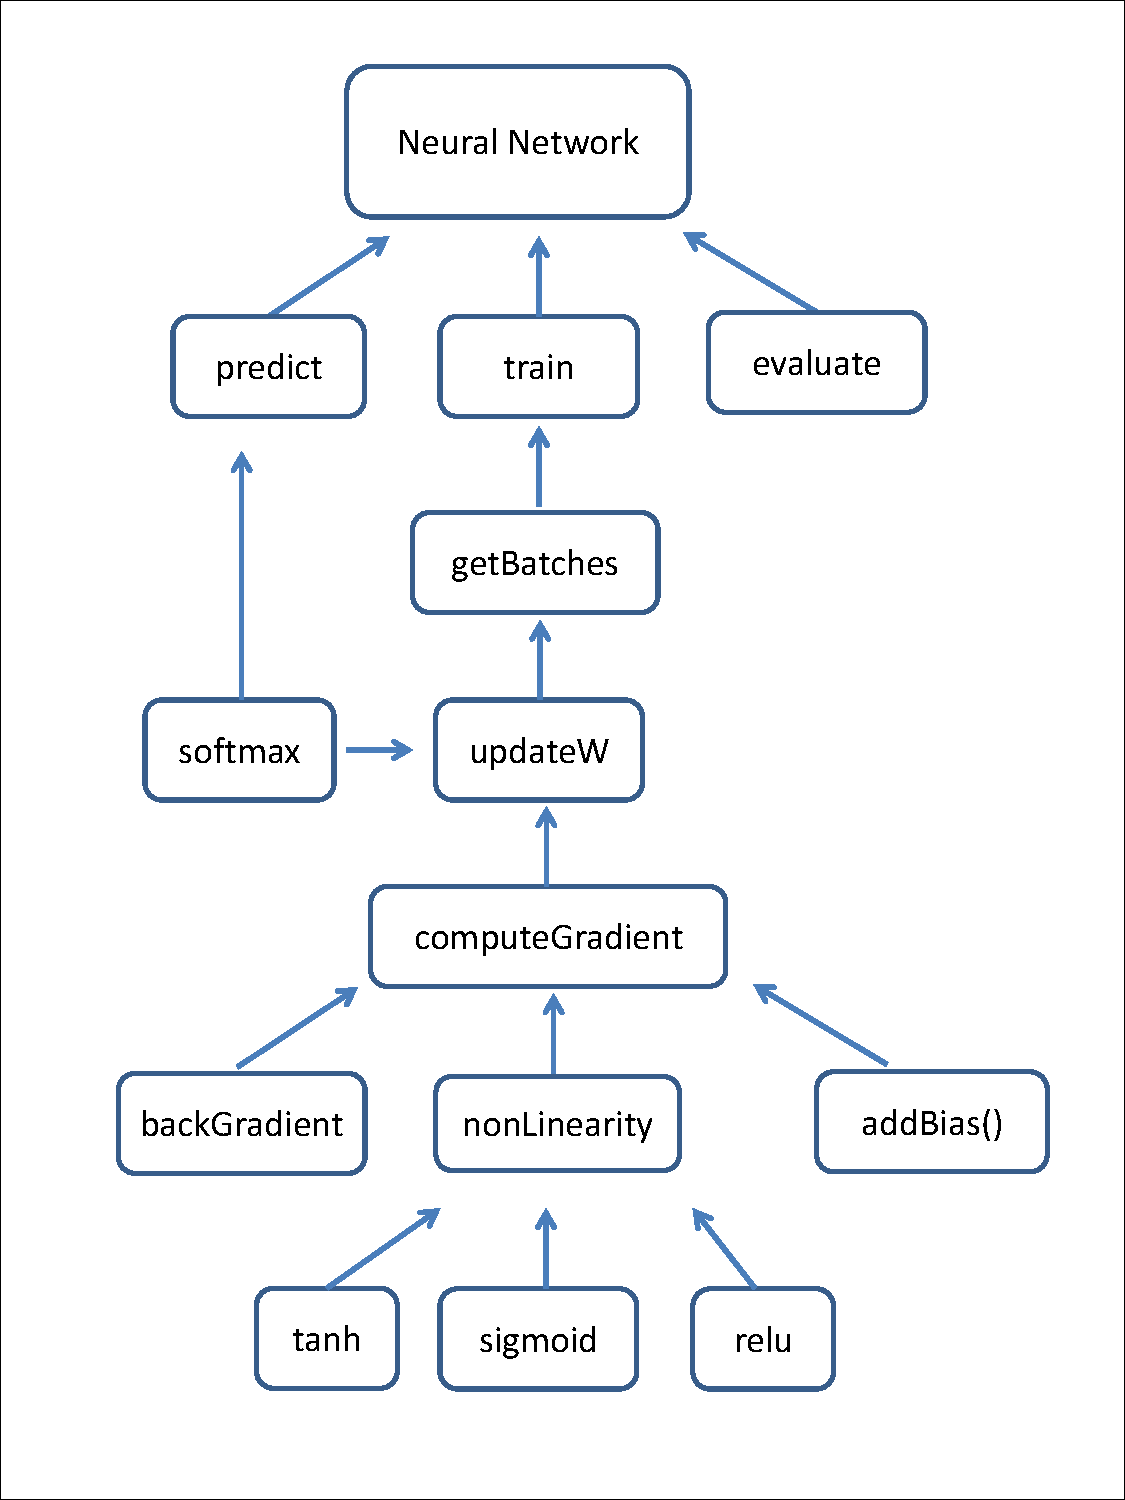
\includegraphics[width=0.7\textwidth]{./figures/ECE544hw2.pdf}\
\caption{\label{fig:structure} Algorithm Structure}
\end{figure}

(2). The whole program has train, predict, evaluate, getBatches, updateW and computeGradient. These functions are based above each other.

On the hidden nodes, you can choose the activation functions such as Sigmoid, Tanh and ReLU functions. The final output layer is calculated using Softmax function. On the back-propagation part, we choose negative log likelihood loss and update the weight one by one.

Due to the large parameters and many training set, we choose mini-batch gradient descent for optimization. On each global iteration, the training set is randomly shuffled and then divided into different batches according predefined batch size. In this work, we studied the influence of different batch sizes, the result will be discussed in next section.

The whole architecture of this part is a fully connected feed-forward multi-layer neural network. Besides the input layer, there are two hidden layers which have same hidden nodes, and the final output layer has 9 nodes corresponding to 9 different labels. 

In the part, since we set the bias term to be 1 for all models and treat bias as an additional dimension, learning rate is one important hyper-parameter. During the experiment, we find that, the learning rate cannot be too large and will be different for different models and different hidden nodes. For example, the learning rate for ReLU activation function is almost always smaller than the learning rate for Sigmoid and Tanh activation function. Specifically, for this work, we choose around 0.6 for ReLU function, 0.3 for Sigmoid function and 0.3 for Tanh function.\\

(3). The total number of weights is different for different hidden nodes. Here, we show two numbers for the case that there are 10 hidden nodes and 50 hidden nodes.

When there are 10 hidden nodes:
$$ \# \  weights = (1120 + 1) \times 10 + (10 + 1) \times 10 + (10 + 1) \times 9 = 11419 $$

When there are 50 hidden nodes:
$$ \# \  weights = (1120 + 1) \times 50 + (50 + 1) \times 50 + (50 + 1) \times 9 = 59059 $$

\noindent {\bf Note}: here we set bias to be 1 all the time and treat bias as an additional dimension.


\subsection*{\large 2. Results}

(1). In this section, we change the hidden nodes from 10 to 50, and choose batch size to be 50, through choosing different activation functions, we find that:\\

\indent For Sigmoid function, with 50 hidden nodes, we can get the highest testing accuracy.\\

\noindent In this case, the training accuracy is $83.67\%$ and the testing accuracy is $46.31\%$. \\

\noindent {\bf Note}: here the highest testing accuracy is chosen based the cross validation, in other words, the development set accuracy. The testing accuracy is calculated on the evaluation set. With enough iterations, the training accuracy can always reach $95\%$ or higher.\\

(2). In Table \ref{table:trainAcc} and Table \ref{table:testAcc}, we have listed the training accuracy and testing accuracy for all combinations between nonlinearities and number of hidden nodes. 

\begin{table}[H]
	\centering
	\caption{Comparison of training accuracy}
	\label{table:trainAcc}	
	\begin{tabular}{c | c | c | c }
		\hline \hline
		Activation Function		&	ReLU	& 	Sigmoid		&	 Tanh 	\\[0.1cm]
		\hline
		(10, 10) hidden nodes	&	66.42\%	&	57.25\%		&	 63.16\% \\[0.1cm]
		(20, 20) hidden nodes	&	87.94\%	&	76.72\%		&	 59.21\% \\[0.1cm]
		(30, 30) hidden nodes	&	60.71\%	&	78.08\%		&	 75.35\% \\[0.1cm]
		(40, 40) hidden nodes	&	56.84\%	&	83.69\%		&	 77.91\% \\[0.1cm]
		(50, 50) hidden nodes	&	69.90\%	&	83.67\%		&	 79.72\% \\[0.1cm]
		\hline	
	\end{tabular}
\end{table}

\begin{table}[H]
	\centering
	\caption{Comparison of test accuracy}
	\label{table:testAcc}	
	\begin{tabular}{c | c | c | c }
		\hline \hline
		Activation Function		&	ReLU	& 	Sigmoid		&	 Tanh 	\\[0.1cm]
		\hline
		(10, 10) hidden nodes	&	39.38\%	&	43.01\%		&	 41.03\% \\[0.1cm]
		(20, 20) hidden nodes	&	43.34\%	&	46.09\%		&	 44.44\% \\[0.1cm]
		(30, 30) hidden nodes	&	43.23\%	&	44.44\%		&	 44.11\% \\[0.1cm]
		(40, 40) hidden nodes	&	35.42\%	&	45.10\%		&	 46.09\% \\[0.1cm]
		(50, 50) hidden nodes	&	40.70\%	&	46.31\%		&	 43.01\% \\[0.1cm]
		\hline	
	\end{tabular}
\end{table}

(3). During the experiment, we also noticed that the running time for each inner iteration varies with batch size and number of hidden nodes, as well as activation functions. In Table \ref{table:time}, we have listed the averaged running for different activation functions and different number of hidden nodes.

\begin{table}[H]
	\centering
	\caption{Average time for one iteration (in seconds)}
	\label{table:time}	
	\begin{tabular}{c | c | c | c }
		\hline \hline
		Activation Function		&	ReLU	& 	Sigmoid		&	 Tanh 	\\[0.1cm]
		\hline
		(10, 10) hidden nodes	&	0.00067	&	0.00309		&	 0.00509 \\[0.1cm]
		(20, 20) hidden nodes	&	0.00073	&	0.00330		&	 0.00535 \\[0.1cm]
		(30, 30) hidden nodes	&	0.00082	&	0.00352		&	 0.00555 \\[0.1cm]
		(40, 40) hidden nodes	&	0.00092	&	0.00366		&	 0.00582 \\[0.1cm]
		(50, 50) hidden nodes	&	0.00105	&	0.00383		&	 0.00614 \\[0.1cm]
		\hline	
	\end{tabular}
\end{table}

It is easy to notice that, ReLU function takes less time than Sigmoid and Tahn function. And with more hidden nodes, the running time becomes larger.

In addition, we also studied the influence of batch size on running time. Through changing the batch size in 50, 100, 150, 200, 250 and 300, we find that with larger batch size, the running time for one iteration becomes larger.\\

(4). In this section, using the best model we have got (as mentioned above), we can calculate the confusion matrix for training and testing set. The training classification confusion matrix and testing classification confusion matrix are shown in Figure \ref{fig:trainMatrix} and Figure \ref{fig:testMatrix}.

Note: the function to plot the confusion matrix is modified based on some online example.

\begin{figure}[H]
\centering
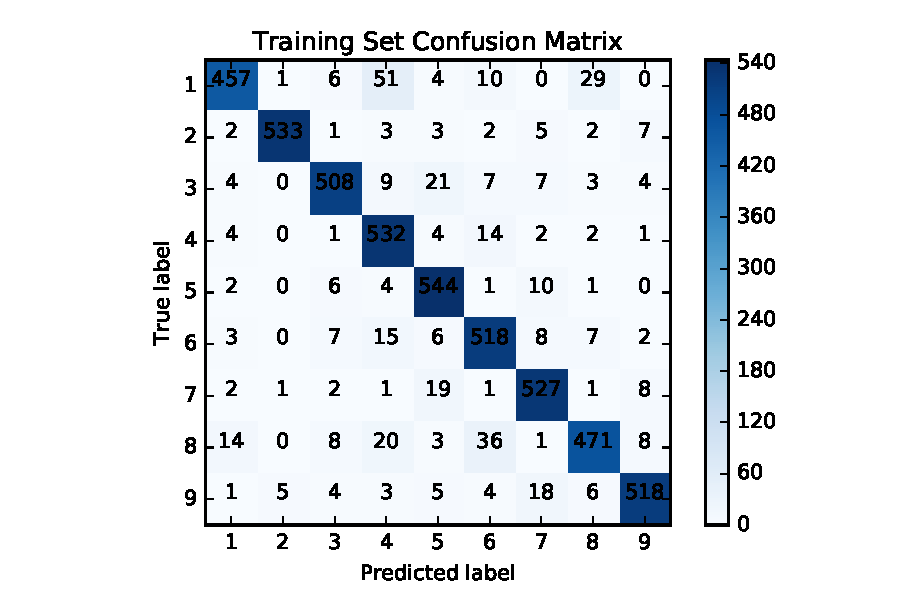
\includegraphics[width=0.9\textwidth]{./figures/trainMatrix.pdf}\
\caption{\label{fig:trainMatrix} Training Set Confusion Matrix}
\end{figure}


\begin{figure}[H]
\centering
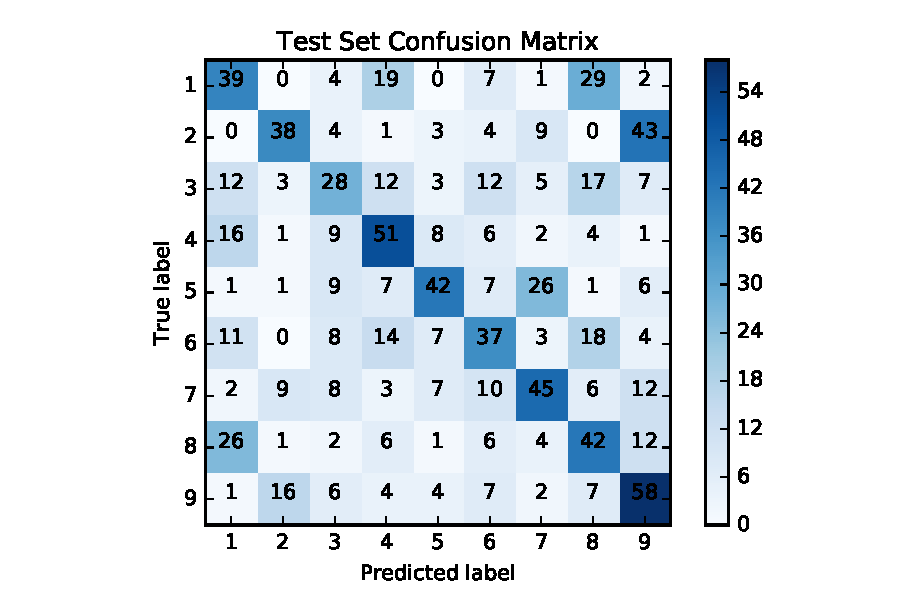
\includegraphics[width=0.9\textwidth]{./figures/testMatrix.pdf}\
\caption{\label{fig:testMatrix} Testing Set Confusion Matrix}
\end{figure}


\newpage
\section*{\Large III. TensorFlow}

\subsection*{\large 1. Methods}

(1). In this section, we use TensorFlow to build a TDNN model following the architecture proposed by Waibel, Hanazawa, Hinton, Shikano and Lang to perform 9 class classification. \\

\noindent At first, we followed the procedure in the literature, choosing the following network architecture:\\
\indent Input Layer: (J=16, N=2)\\
\indent Hidden Layer 1: (J=8, N=4)\\
\indent Hidden Layer 2: (J=3)\\
\indent Output Layer: fully connected feed-forward neural network with 9 output.\\

\noindent More specifically, we choose ReLU function as the activation function. For the final layer, we first flatten the output of hidden layer 2 to be one column vector and train a fully connected neural network to classify 9 classes. And final output is calculated through Softmax function and the loss function is negative log likelihood loss and train the model through ADAM optimizer. The learning rate is chosen to be 0.002 and the batch size is setting to be 50.

The used TensorFlow function includes: tf.reshape(), tf.nn.relu(), tf.nn.softmax(), tf.nn.conv2d() and so on. The final training accuracy is $55.91\%$ and final testing accuracy is $45.76\%$. \\

\noindent {\bf Note: } Here, one important thing is that, in each iteration, we don't train the model on all the batches. Instead, on each iteration, we first randomly shuffle the training set and split them into different subsets according to given batch sizes. Then, we select the first 5 batches to perform mini-batch training rather than using all batches to train the model.\\ 

(2). Besides the above model, we also tried different models, for example, in the above model, the output of the second hidden layer is an image with dimension (64, 3). However, since we have 9 classed, one direct idea is the change the output from (64, 3) to (64, 9), and then perform fully connected feed-forward neural network. Our result shows that, this change can improve the testing accuracy from $45.76\%$ to $52.25\%$. Besides, the second hidden layer, we also tried to use different filters, such as more delay in input layer and/or less delay in first hidden layer. Some changes have clear influence, but some changes have little influence.

In addition, we also noticed that in the original paper, the author setting the final output to be the Sigmoid function of the sum of the output of hidden layer 2. Here, we also edit our model so that the final output is not a fully connected feed-forward neural network. Instead, since the output of second hidden layer has dimension (64, 9). We use the mean value of each column as the input to final output layer and use Softmax function to perform 9 class prediction. In this model, we noticed that our model has testing accuracy of $57.32\%$.\\

\noindent {\bf Note: } During the training process, we also noticed that some of our model is sensitive to the initialization. The final output accuracy may varies a lot. The reported accuracy mentioned above is the highest accuracy we ever get. (All testing accuracy is determined through development set, rather than decided directly.)\\

(3). In the original TDNN model we set:\\
\indent Input Layer: (J=16, N=2)\\
\indent Hidden Layer 1: (J=8, N=4)\\
\indent Hidden Layer 2: (J=3)\\
\indent Output Layer: fully connected feed-forward neural network with 9 output.\\
So, we can calculate the total number of weights as follows:
$$ \# \  weights = 16 \times 3 \times 8 + 8 \times 5 \times 3 + 64 \times 3 \times 9 = 2232 $$

\noindent {\bf Note: } Here, we didn't consider bias as the additional weights, if bias is considered, then:
$$ \# \  weights = 16 \times 3 \times 8 + 8 + 8 \times 5 \times 3 + 3 + 64 \times 3 \times 9 + 9 = 2252 $$

(4). For the original TDNN model, at the first hidden layer, the activation dimensions are:
$$ 3 \times 16 + 1 = 49 $$

At the second hidden layer, the activation dimensions are:
$$ 5 \times 8 + 1 = 41 $$

At the final output layer, since we use the fully connected neural network, the activation dimensions are:
$$ 64 \times 3 + 1 = 193 $$

(5). The used TensorFlow function includes: tf.reshape(), tf.nn.relu(), tf.nn.softmax(), tf.nn.conv2d() and so on. Specifically, for tf.nn.conv2d(), we choose "VALID" mode, as shown in line 54 of TensorFlow.py. In addition, we initialize the weight variable through tf.truncated{\_}normal() and initialize the b variable to be constant 0.1.

The overall structure of the code is simple, in file named TenforFlow.py, there are generally 4 parts. In the first part, we load the data and define some helper functions. Then, in the second part, we apply the model as required by the course website, where: \\
\indent Input Layer: (J=16, N=2)\\
\indent Hidden Layer 1: (J=8, N=4)\\
\indent Hidden Layer 2: (J=3)\\
\indent Output Layer: fully connected feed-forward neural network with 9 output.\\

On the third part, we used a flexible model, where you can change the filter size, learning rate and so on. On the last part, we used a similar model similar to part 2, but on the final output layer, we don't use a fully connected feed-forward neural network from hidden layer 2 to output layer, instead, we use the mean value of each dimension from hidden layer 2 as the input to final output layer, and then perform Softmax() function for 9 class classification. This is similar to the original model described in the paper.

On each part of part 2, 3 and 4, the overall structure of the code is similar. First we define the hyper-parameters such as learning rate. Then, we create the tensorFlow session and create some placeholders to hold the variables. Then through define the weight filter and bias term for each layer, we create all the variables. Next, we define the loss and accuracy. Through selecting appropriate batches, we start training the model and use the trained model to calculate the training accuracy and development accuracy. Finally, we find the best model through development set and apply the model on the evaluation set and plot the convergence curve and confusion matrix.

\subsection*{\large 2. Results}

(1). In this part, following the procedure described above, we calculate the training and testing accuracy for TDNN model. 

\begin{table}[H]
	\centering
	\caption{Training and testing accuracy for TDNN model}
	\label{table:TDNNacc}	
	\begin{tabular}{c | c}
		\hline \hline
		Used Set  		&	Accuracy \\[0.1cm]
		\hline
		Training Set	&	55.91\%	\\[0.1cm]
		Testing Set		&	45.76\%	\\[0.1cm]
		\hline	
	\end{tabular}
\end{table}


(2). In this part, following the procedure described above, we calculate the training and testing accuracy for best TDNN model we have got. 

\begin{table}[H]
	\centering
	\caption{Training and testing accuracy for best model}
	\label{table:BESTacc}	
	\begin{tabular}{c | c}
		\hline \hline
		Used Set  		&	Accuracy \\[0.1cm]
		\hline
		Training Set	&	67.64\%	\\[0.1cm]
		Testing Set		&	57.32\%	\\[0.1cm]
		\hline	
	\end{tabular}
\end{table}


(3). In this part, the training and testing classification confusion matrix for the TDNN model are shown in Figure \ref{fig:TDNNtrainMatrix} and Figure \ref{fig:TDNNtestMatrix}. 

\begin{figure}[H]
\centering
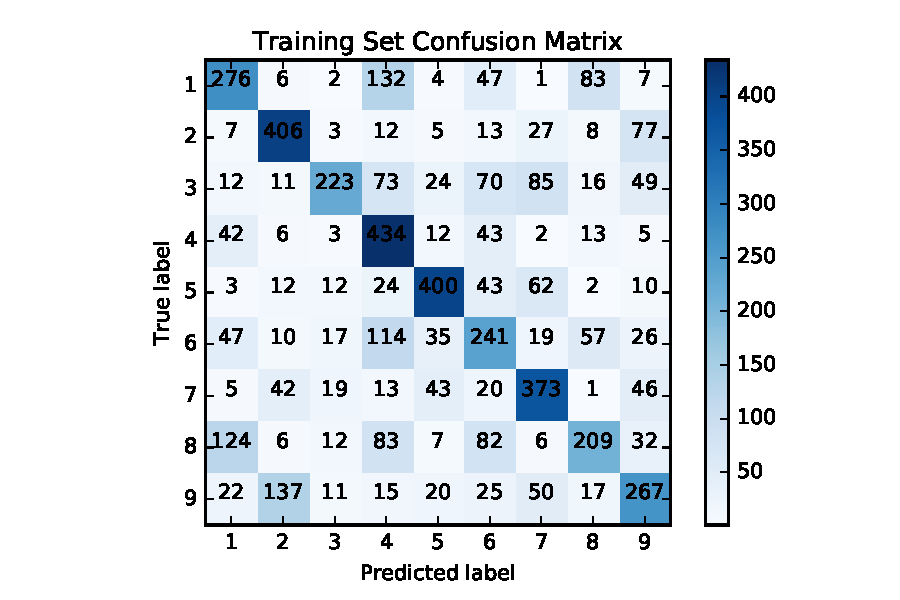
\includegraphics[width=0.9\textwidth]{./figures/requiredTDNNtrain.pdf}\
\caption{\label{fig:TDNNtrainMatrix} Training Set Confusion Matrix for TDNN model}
\end{figure}


\begin{figure}[H]
\centering
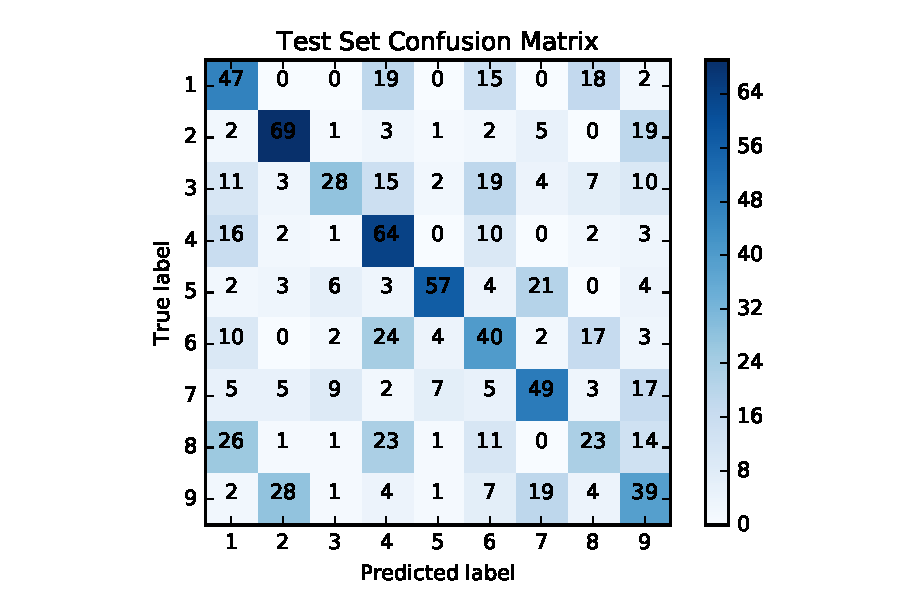
\includegraphics[width=0.9\textwidth]{./figures/requiredTDNNtest.pdf}\
\caption{\label{fig:TDNNtestMatrix} Testing Set Confusion Matrix for TDNN model}
\end{figure}


The training and testing classification confusion matrix for the best TDNN model are shown in Figure \ref{fig:BESTtrainMatrix} and Figure \ref{fig:BESTtestMatrix}. 

\begin{figure}[H]
\centering
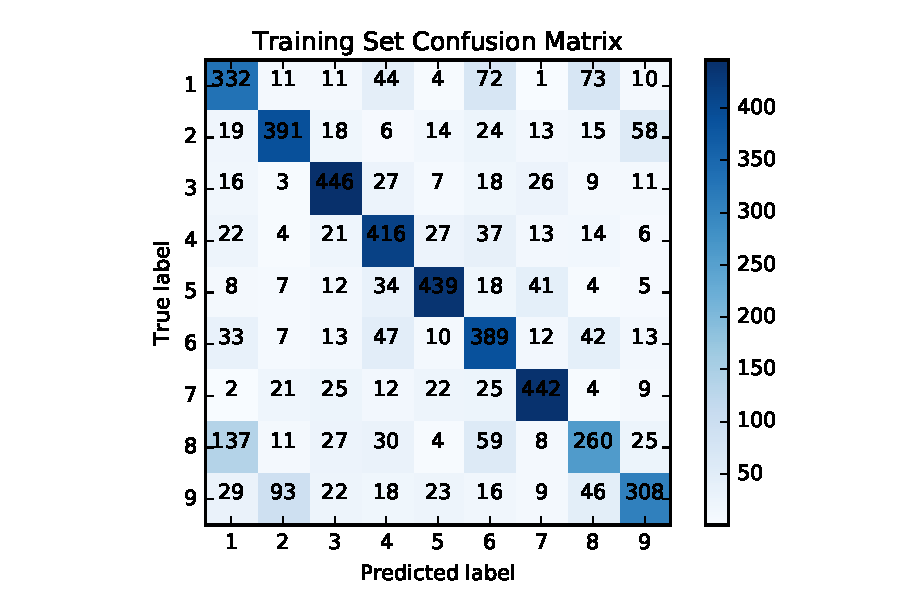
\includegraphics[width=0.9\textwidth]{./figures/originalTDNNtrain.pdf}\
\caption{\label{fig:BESTtrainMatrix} Training Set Confusion Matrix for best model}
\end{figure}


\begin{figure}[H]
\centering
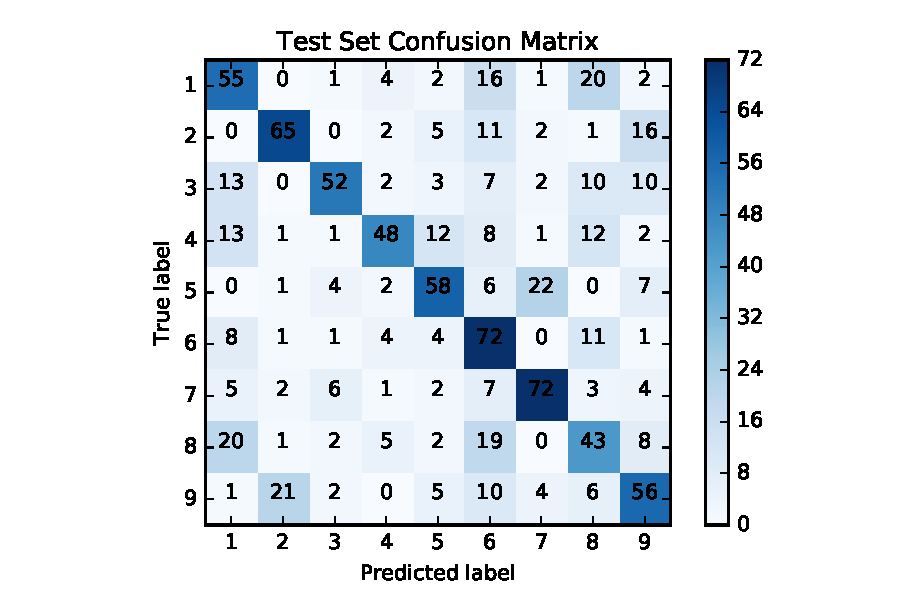
\includegraphics[width=0.9\textwidth]{./figures/originalTDNNtest.pdf}\
\caption{\label{fig:BESTtestMatrix} Test Set Confusion Matrix for best model}
\end{figure}


\clearpage

\end{document}

